\documentclass[conference]{IEEEtran}
\usepackage{cite}
\usepackage{amsmath,amssymb,amsfonts}
\usepackage{algorithmic}
\usepackage{graphicx}
\usepackage{textcomp}
\usepackage{xcolor}
\usepackage{tikz}
\usepackage{booktabs}
\usepackage{multirow}
\usepackage{float}
\usepackage{nomencl}
\usepackage{url}

% ==========================================
% TIKZ SETUP
% ==========================================
\usetikzlibrary{shapes.geometric, arrows, positioning, calc, fit, backgrounds, shapes.misc, decorations.pathmorphing}
\tikzset{
  layer/.style={
    rectangle, 
    minimum width=7cm, 
    minimum height=0.7cm, 
    text centered, 
    draw=black, 
    fill=blue!5,
    font=\small\bfseries
  },
  payload/.style={
    font=\footnotesize\itshape,
    align=center
  },
  arrow/.style={
    thick, 
    ->, 
    >=stealth
  },
  forbidden/.style={
    thick, 
    ->, 
    >=stealth,
    red,
    dashed
  },
  cross/.style={
    cross out, 
    draw=red, 
    minimum size=7pt, 
    inner sep=0pt, 
    outer sep=0pt,
    very thick
  },
  failnode/.style={
    rectangle,
    rounded corners,
    draw=red!80,
    fill=red!10,
    text width=3.5cm,
    text centered,
    font=\footnotesize\bfseries,
    minimum height=0.8cm
  },
  safenode/.style={
    rectangle,
    rounded corners,
    draw=green!60!black,
    fill=green!5,
    text width=3.5cm,
    text centered,
    font=\footnotesize\bfseries,
    minimum height=0.8cm
  },
  failarrow/.style={
    thick,
    ->,
    >=stealth,
    red,
    decorate,
    decoration={snake, amplitude=.4mm, segment length=2mm, post length=1mm}
  },
  safearrow/.style={
    thick,
    ->,
    >=stealth,
    blue!70!black
  }
}

\begin{document}

% ==========================================
% TITLE
% ==========================================
\title{ScholarMaster: A Layered Edge-Native Architecture for Real-Time Context-Aware Intelligent Systems}

% ==========================================
% AUTHORS
% ==========================================
\author{
\IEEEauthorblockN{
Polisetti Narendra\IEEEauthorrefmark{1}, 
Suresh Kumar Sreedharan\IEEEauthorrefmark{2}, 
Vijaya Raju Motru\IEEEauthorrefmark{3}, and 
Praveena Mallampalli\IEEEauthorrefmark{4}
}
\IEEEauthorblockA{\textit{Swarnandhra College of Engineering \& Technology (Autonomous)}\\
Narsapur, Andhra Pradesh, India \\
\IEEEauthorrefmark{1}ORCID: 0009-0002-6355-138X, 
\IEEEauthorrefmark{2}ORCID: 0000-0001-9912-5927 \\
\IEEEauthorrefmark{3}vijayaraju.m@gmail.com, 
\IEEEauthorrefmark{4}praveena.iduri@gmail.com}
}

\maketitle

% ==========================================
% ABSTRACT
% ==========================================
\begin{abstract}
Modern intelligent systems increasingly operate under strict real-time, privacy, and resource constraints, particularly in edge-native environments. While individual advances in perception, inference, and control have improved component-level performance, the absence of a unified architectural framework frequently yields tightly coupled monoliths that defy independent validation. 

ScholarMaster treats architectural decomposition itself as a verifiable systems property rather than a software engineering convenience. This paper consolidates findings from a multi-paper research program into a coherent edge-native framework, decomposing the context-aware pipeline into isolated domains: sensing, geometric abstraction, probabilistic interpretation, logical evaluation, and control. 

By enforcing strict abstraction admissibility between these stages, the architecture substantially constrains cross-layer leakage. Modularity emerges as a direct consequence of these boundary invariants. Drawing on experience from independently validated subsystem studies, we demonstrate how deterministic composition offers significant advantages over monolithic fusion when interpretability, fault isolation, and deployment auditability are the primary operational metrics.
\end{abstract}

% ==========================================
% KEYWORDS
% ==========================================
\begin{IEEEkeywords}
System Architecture, Edge-Native, Boundary Invariants, Deterministic Composition, Abstraction Admissibility, Fault Containment.
\end{IEEEkeywords}

% ==========================================
% I. INTRODUCTION
% ==========================================
\section{Introduction}

The dominant thesis of this paper is that \textbf{architectural boundary invariants can transform decomposition itself into a verifiable systems property for edge-native intelligent systems.} This manuscript functions strictly as a systems-architecture paper analyzing edge-native structural composition, not a generalized intelligent-campus framework or a policy manifesto.

\subsection{Operational Fragility in End-to-End Intelligent Systems}
Deploying intelligent systems within institutional cyber-physical environments \cite{b1, b5, b15} involves managing tightly coupled operational constraints \cite{b6}. Monolithic edge pipelines frequently fail under incremental evolution. Tightly coupled representations accumulate hidden dependencies; subsystem upgrades destabilize unrelated logic; audit reconstruction becomes operationally infeasible; and implicit cross-layer assumptions grow over time. The core issue is architectural entanglement, not merely implementation complexity.

Over the course of developing the ScholarMaster subsystem ecosystem, these architectural failure patterns became apparent \cite{b2, b13, b16}:
\begin{enumerate}
    \item \textbf{End-to-End Monoliths:} Optimization pressures favor direct, opaque coupling. While performant in static benchmarks, these pipelines proved brittle under incremental evolution \cite{b17}.
    \item \textbf{Cloud-Modular Dependencies:} Offloading reasoning introduces temporal jitter and privacy exposure \cite{b3, b18}.
    \item \textbf{Loose Event-Driven Buses:} Exhibit ``abstraction drift''---components operating on conflicting temporal views accumulate synchronization inconsistencies.
\end{enumerate}

\subsection{Subsystem Scope and Canonical Separation}
Within the ScholarMaster architecture, this specific subsystem explicitly defines architectural strata, formalizes abstraction admissibility, and constrains cross-layer interaction. This subsystem does NOT implement probabilistic engagement interpretation (Paper 2), perform geometric sensing (Paper 3), execute runtime verification proofs (Paper 18), coordinate orchestration policy (Paper 9), or manage cryptographic provenance (Paper 8).

The ScholarMaster architecture emerged from the recognition that decomposition must function as an enforceable operational constraint. This work consolidates the architectural understanding that evolved across the research program, synthesizing independently developed subsystem formalizations into a coherent reference framework.

% ==========================================
% II. RELATED ARCHITECTURAL PARADIGMS
% ==========================================
\section{Related Architectural Paradigms}
The architectural decisions underlying ScholarMaster are best understood against the structural limitations of existing intelligent system paradigms. Three dominant models have shaped edge-intelligent system design, and each reveals a distinct category of decomposition failure relevant to institutional cyber-physical environments.

End-to-end monolithic pipelines \cite{b7} remain prevalent due to their implementation simplicity and throughput efficiency. Their central weakness is representational entanglement: perception, reasoning, and execution share opaque intermediate representations, making it difficult to attribute a behavioral anomaly to a specific functional origin. When such a system produces an incorrect decision, isolating whether the fault lies in sensory interpretation, logical evaluation, or control dispatch typically requires global pipeline introspection---a cost that scales poorly under institutional audit requirements.

Cloud-native microservice architectures \cite{b4, b14} address this coupling through network-level decomposition, but introduce a different failure mode. In edge environments, serialization and network transit overhead produces temporal jitter that undermines the determinism required for cyber-physical synchronization \cite{b19}. More subtly, loosely constrained service interfaces allow hidden semantic dependencies to emerge across layers, recreating at the API level the same entanglement that monoliths exhibit at the memory level.

Event-driven distributed pipelines \cite{b9} partially address both scalability and modularity, yet they introduce synchronization drift: components operating on conflicting temporal snapshots of the environment accumulate inconsistent logical states. Without explicit temporal contracts, these inconsistencies remain latent until they surface as coordination failures during high-load or degraded operating conditions.

A common thread across these paradigms is that none treat decomposition boundaries as architecturally enforceable invariants. Boundaries exist as development conventions rather than structural constraints, and they erode under optimization pressure. Across the subsystem studies comprising the ScholarMaster program, this erosion was observed repeatedly during independent module validation. The architecture responds by elevating boundary enforcement to a first-class systems property (Table~\ref{tab:related_work}), prioritizing deterministic composition, abstraction admissibility, and long-term auditability over raw computational throughput.

\begin{table}[htbp]
\caption{Architectural Paradigm Comparison}
\label{tab:related_work}
\centering
\begin{tabular}{@{}p{2.5cm} p{2.5cm} p{2.8cm}@{}}
\toprule
\textbf{Paradigm} & \textbf{Primary Weakness} & \textbf{ScholarMaster Alternative} \\
\midrule
Monolithic AI & Opaque coupling & Boundary invariants \\
\addlinespace
Microservice AI & Weak determinism & Edge-native memory confinement \\
\addlinespace
Event-Driven & Synchronization drift & Strict upward abstraction admissibility \\
\bottomrule
\end{tabular}
\end{table}

% ==========================================
% III. DESIGN PRINCIPLES AND FORMALISMS
% ==========================================
\section{Boundary Invariants and Formalisms}
Several operational tensions emerged during layered decomposition of the ScholarMaster subsystems. Resolving these tensions led to a set of boundary invariants that enforce abstraction admissibility across the stack. Decomposition is treated as an enforceable operational constraint, not merely a development preference. Boundaries are enforced structurally rather than organizationally, explicitly distinguishing interface contracts, abstraction admissibility, ownership isolation, and semantic leakage prevention.

\subsection{Abstraction Admissibility}
Modularity is maintained by constraining each layer $L_i$ to a bounded transformation:
\begin{equation}
L_i : X_i \to X_{i+1}
\end{equation}
where $X_i$ represents the \textit{minimal abstraction admissible} for upward propagation. Higher layers consume strictly immutable abstractions. A sensing layer may output geometric coordinates, but it is structurally incapable of emitting a logical predicate. This constraint prevents higher-level logic from becoming implicitly dependent on lower-level implementation details \cite{b12, b20}.

\subsection{Edge-Native Memory Confinement}
Computation resolves entirely on localized, volatile hardware. By severing cloud dependencies, the architecture eliminates network jitter and natively enforces data sovereignty. Earlier subsystem formalizations revealed that treating all external network paths as hostile or unavailable was essential for ensuring critical path logic operates in functional isolation.

\subsection{Deterministic Composition}
Determinism emerges from constrained architectural interaction, not merely synchronous execution. Predictability is achieved by treating lower-layer outputs as immutable, deterministic inputs. Skip-layer access introduces semantic instability and is explicitly prohibited. Traceability emerges from constrained upward propagation. The system's emergent behavior consequently becomes formally traceable within the defined bounds, eliminating the opacity associated with end-to-end deep learning pipelines where intermediate representations lack defined semantics.

% ==========================================
% IV. THE SCHOLARMASTER REFERENCE MODEL
% ==========================================
\section{The ScholarMaster Reference Model: A 4-Stratum Architecture}
The architecture is structured into four distinct strata, each representing a discrete domain of operational responsibility and data sensitivity. This stratification ensures that raw physical observations never mix with institutional governance logic.

\begin{itemize}
    \item \textbf{Physics Stratum (L1-L2):} Manages raw sensing and geometric abstraction. Subsystems in this stratum extract objective coordinates while remaining agnostic to institutional identity.
    \item \textbf{Logic Stratum (L3-L4):} Converts geometric abstractions into probabilistic states and logical predicates. This stratum handles uncertainty propagation and enforces the Boolean evaluation rules governing system behavior.
    \item \textbf{Verification Stratum (L5-L6):} Ensures the system operates within its temporal and formal bounds, enforcing sub-millisecond scheduling and architectural isolation.
    \item \textbf{Governance Stratum (L7-L8):} Handles auditing, privacy preservation, and institutional reporting, managing the SHA-256 chains that allow auditing without exposing raw data.
\end{itemize}

Figure \ref{fig:layers} visualizes the required abstraction contracts and illustrates the architectural hazards of bypassing them. 

\begin{figure}[htbp]
\centering
\resizebox{0.48\textwidth}{!}{
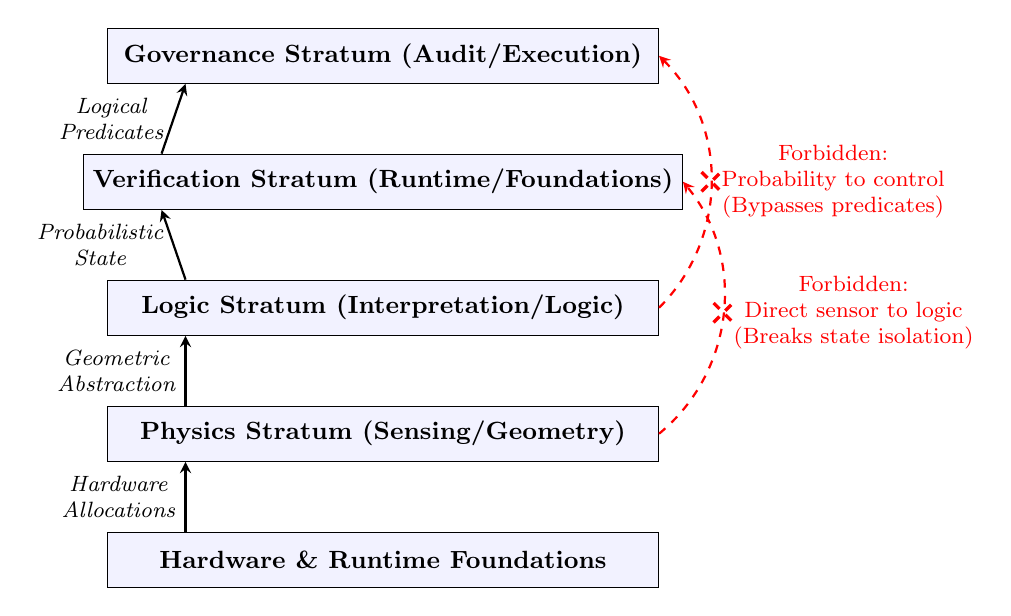
\begin{tikzpicture}[node distance=1.6cm]
  
  % Layers
  \node (L0) [layer] {Governance Stratum (Audit/Execution)};
  \node (L1) [layer, below of=L0] {Verification Stratum (Runtime/Foundations)};
  \node (L2) [layer, below of=L1] {Logic Stratum (Interpretation/Logic)};
  \node (L3) [layer, below of=L2] {Physics Stratum (Sensing/Geometry)};
  \node (L4) [layer, below of=L3] {Hardware \& Runtime Foundations};

  % Valid Arrows (Left Side)
  \draw[arrow] (L4.north west) ++(1cm,0) -- node[left, payload] {Hardware\\Allocations} ([xshift=1cm]L3.south west);
  \draw[arrow] (L3.north west) ++(1cm,0) -- node[left, payload] {Geometric\\Abstraction} ([xshift=1cm]L2.south west);
  \draw[arrow] (L2.north west) ++(1cm,0) -- node[left, payload] {Probabilistic\\State} ([xshift=1cm]L1.south west);
  \draw[arrow] (L1.north west) ++(1cm,0) -- node[left, payload] {Logical\\Predicates} ([xshift=1cm]L0.south west);

  % Invalid Arrows (Right Side - Cross Layer Leakage)
  \draw[forbidden] (L3.east) to[bend right=45] node[right, align=center, text=red, font=\footnotesize] {Forbidden:\\Direct sensor to logic\\(Breaks state isolation)} node[midway, cross] {} (L1.east);
  
  \draw[forbidden] (L2.east) to[bend right=45] node[right, align=center, text=red, font=\footnotesize] {Forbidden:\\Probability to control\\(Bypasses predicates)} node[midway, cross] {} (L0.east);

\end{tikzpicture}
}
\caption{The ScholarMaster Layered Architecture. Allowed interfaces mandate progressive abstraction (left). Lateral or skip-level communication is explicitly forbidden to prevent cross-layer leakage (right).}
\label{fig:layers}
\end{figure}

\subsection{Constraint-First Architectural Synthesis (CFAS)}
The ScholarMaster architecture evolved through a Constraint-First Architectural Synthesis (CFAS) methodology. CFAS operates as an inversion of conventional AI-system construction. Boundary constraints precede feature synthesis, subsystem admissibility is evaluated before integration, and architectural survivability outweighs short-term throughput optimization. Rather than beginning with a feature set and attempting to bolt on privacy and real-time guarantees, the process first established the boundary invariants ($B_i$) and then synthesized the functional features that could exist within those constraints. This inversion of the typical design sequence emerged from early prototyping experience, where feature-first approaches repeatedly produced architectures that required expensive post-hoc privacy remediation.

\subsection{Schema-Constrained Semantic Firewalls}
Schema constraints enforce abstraction admissibility, not absolute security guarantees. The architecture enforces an "Irreversibility Boundary" through schema-constrained semantic firewalls. By utilizing strictly typed serialization (e.g., Protobuf), the system restrains representational leakage and abstraction narrowing reduces downstream semantic dependency, making it structurally impossible to pass a raw image tensor or an absolute coordinate across a layer boundary. For example, the interface between the Sensing and Reasoning layers is constrained to categorical IDs and logical spatial zones, precluding the possibility of identity leakage through high-dimensional raw features.

% ==========================================
% V. CROSS-LAYER CONSISTENCY
% ==========================================
\section{Cross-Layer Consistency and the Research Ecosystem}
The ScholarMaster ecosystem decomposes architectural responsibility into independently verifiable domains spanning sensing, reasoning, runtime enforcement, and governance. This decomposition evolved organically as subsystem complexity grew: what began as a monolithic prototype progressively fractured into distinct ownership domains as operational tensions between layers became apparent. Each subsystem now evolves under independently auditable constraints while preserving global operational consistency. Individual subsystem formalizations are documented across the broader ScholarMaster research program (Table \ref{tab:subsystem_mapping}).

\begin{table}[htbp]
\caption{Subsystem Ownership Mapping}
\label{tab:subsystem_mapping}
\centering
\begin{tabular}{@{}ll@{}}
\toprule
\textbf{Subsystem Domain} & \textbf{Primary Formalization Source} \\
\midrule
Vision Geometry & SM-P3 \\
Acoustic Sensing & SM-P6 \\
Probabilistic Interpretation & SM-P2 \\
Logical Evaluation & SM-P4 \\
Runtime Scheduling & SM-P20 \\
Formal Foundations & SM-P21 \\
Privacy Governance & SM-P8 \\
Identity Retrieval & SM-P7 \\
Reference Architecture & SM-P18 \\
Threat Modeling & SM-P19 \\
Control Dispatch & SM-P9 \\
State Management & SM-P11 \\
\bottomrule
\end{tabular}
\end{table}

\begin{figure*}[htbp]
\centering
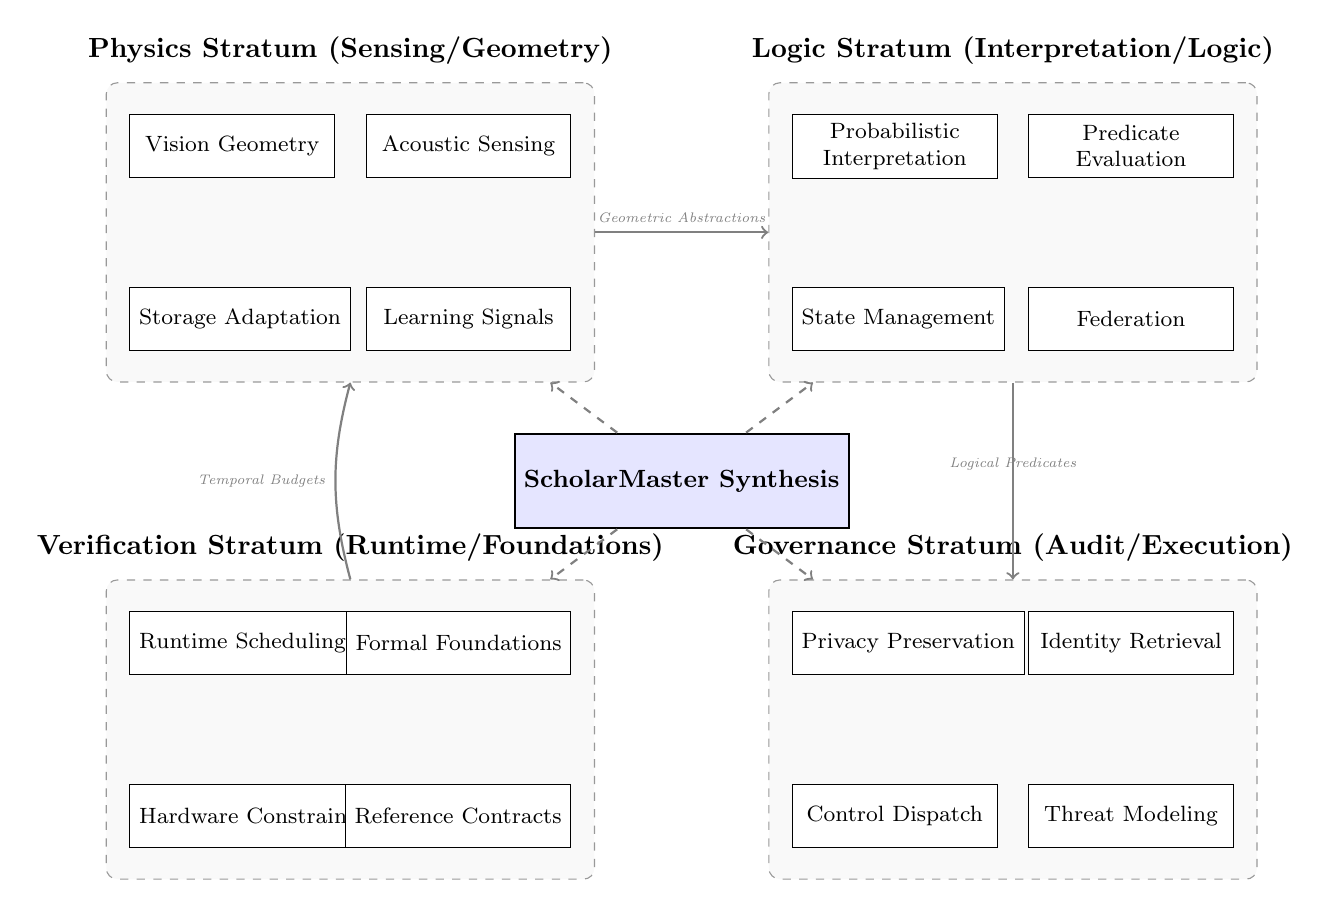
\begin{tikzpicture}[
  group/.style={rectangle, draw=black!40, fill=gray!5, dashed, inner sep=0pt, rounded corners, minimum width=6.2cm, minimum height=3.8cm},
  paper/.style={rectangle, draw=black, fill=white, minimum width=2.6cm, minimum height=0.8cm, font=\footnotesize, align=center}
]

  % PHYSICS STRATUM
  \node (G_sensing) [group] {};
  \node [above=0.1cm of G_sensing.north, font=\bfseries] {Physics Stratum (Sensing/Geometry)};
  
  \node (P3)  [paper, anchor=north west] at ([xshift=0.3cm, yshift=-0.4cm]G_sensing.north west) {Vision Geometry};
  \node (P6)  [paper, anchor=north east] at ([xshift=-0.3cm, yshift=-0.4cm]G_sensing.north east) {Acoustic Sensing};
  \node (P12) [paper, anchor=south west] at ([xshift=0.3cm, yshift=0.4cm]G_sensing.south west) {Storage Adaptation};
  \node (P13) [paper, anchor=south east] at ([xshift=-0.3cm, yshift=0.4cm]G_sensing.south east) {Learning Signals};

  % LOGIC STRATUM
  \node (G_reasoning) [group, right=2.2cm of G_sensing] {}; 
  \node [above=0.1cm of G_reasoning.north, font=\bfseries] {Logic Stratum (Interpretation/Logic)};

  \node (P2)  [paper, anchor=north west] at ([xshift=0.3cm, yshift=-0.4cm]G_reasoning.north west) {Probabilistic\\Interpretation};
  \node (P4)  [paper, anchor=north east] at ([xshift=-0.3cm, yshift=-0.4cm]G_reasoning.north east) {Predicate\\Evaluation};
  \node (P11) [paper, anchor=south west] at ([xshift=0.3cm, yshift=0.4cm]G_reasoning.south west) {State Management};
  \node (P14) [paper, anchor=south east] at ([xshift=-0.3cm, yshift=0.4cm]G_reasoning.south east) {Federation};

  % VERIFICATION STRATUM
  \node (G_runtime) [group, below=2.5cm of G_sensing] {};
  \node [above=0.1cm of G_runtime.north, font=\bfseries] {Verification Stratum (Runtime/Foundations)};

  \node (P20) [paper, anchor=north west] at ([xshift=0.3cm, yshift=-0.4cm]G_runtime.north west) {Runtime Scheduling};
  \node (P21) [paper, anchor=north east] at ([xshift=-0.3cm, yshift=-0.4cm]G_runtime.north east) {Formal Foundations};
  \node (P5)  [paper, anchor=south west] at ([xshift=0.3cm, yshift=0.4cm]G_runtime.south west) {Hardware Constraints};
  \node (P18) [paper, anchor=south east] at ([xshift=-0.3cm, yshift=0.4cm]G_runtime.south east) {Reference Contracts};

  % GOVERNANCE STRATUM
  \node (G_governance) [group, right=2.2cm of G_runtime] {};
  \node [above=0.1cm of G_governance.north, font=\bfseries] {Governance Stratum (Audit/Execution)};

  \node (P8)  [paper, anchor=north west] at ([xshift=0.3cm, yshift=-0.4cm]G_governance.north west) {Privacy Preservation};
  \node (P7)  [paper, anchor=north east] at ([xshift=-0.3cm, yshift=-0.4cm]G_governance.north east) {Identity Retrieval};
  \node (P9)  [paper, anchor=south west] at ([xshift=0.3cm, yshift=0.4cm]G_governance.south west) {Control Dispatch};
  \node (P19) [paper, anchor=south east] at ([xshift=-0.3cm, yshift=0.4cm]G_governance.south east) {Threat Modeling};

  % SYNTHESIS CENTER
  \path (G_sensing.south east) -- (G_governance.north west) coordinate[midway] (center);
  \node (P1) [paper, fill=blue!10, thick, minimum width=3.8cm, minimum height=1.2cm, font=\small\bfseries] at (center) {ScholarMaster Synthesis};

  % ARROW CONNECTIONS
  \draw[->, thick, gray] (G_sensing) -- node[above, font=\tiny\itshape] {Geometric Abstractions} (G_reasoning);
  \draw[->, thick, gray] (G_reasoning) -- node[above, font=\tiny\itshape] {Logical Predicates} (G_governance);
  \draw[->, thick, gray] (G_runtime.north) to[bend left=15] node[left, font=\tiny\itshape] {Temporal Budgets} (G_sensing.south);
  
  \draw[->, thick, gray, dashed] (P1) -- (G_sensing);
  \draw[->, thick, gray, dashed] (P1) -- (G_reasoning);
  \draw[->, thick, gray, dashed] (P1) -- (G_runtime);
  \draw[->, thick, gray, dashed] (P1) -- (G_governance);

\end{tikzpicture}
\caption{The ScholarMaster Research Ecosystem Map. The architecture decomposes architectural responsibility into four independently verifiable strata (Physics, Logic, Verification, Governance). This structural decomposition illustrates how functional boundaries may be enforced without introducing uncontrolled cross-layer leakage.}
\label{fig:ecosystem}
\end{figure*}

\section{Example Operational Trace: Attendance Validation}
To ground the preceding formalism in operational reality, consider a concrete institutional attendance validation event. This trace illustrates the layered traceability that the architecture enforces across a single decision lifecycle.

The journey begins at the \textbf{Sensing Layer}, which extracts raw geometric occupancy abstractions (bounding boxes, skeletal points) from visual and acoustic streams. Crucially, this layer does not know "who" is present or "why"; it merely produces stateless physical coordinates.

These abstractions propagate to the \textbf{Probabilistic Interpretation Layer}, where they are anchored against temporal priors to produce bounded confidence states. This layer determines the likelihood of sustained presence while smoothing out sensory jitter.

The resulting probability state is consumed by the \textbf{Logical Evaluation Layer}, which tests institution-specific predicates—such as duration thresholds or authorized schedule compliance. Only after deterministic predicate satisfaction does the \textbf{Control Layer} emit an operational action, such as updating a ledger or granting access.

At no point does the control layer access raw sensor tensors, nor does the sensing layer interpret institutional policy semantics. If a decision is later questioned, an auditor can reconstruct the exact logical predicate and the specific probabilistic state that triggered it, without needing to re-watch hours of raw video.

% ==========================================
% VI. WHY LAYER VIOLATIONS ARE DANGEROUS
% ==========================================
\section{Architectural Hazards of Cross-Layer Leakage}

Across the subsystem studies, a consistent pattern emerged: the most operationally significant failures in edge-intelligent systems rarely originated from algorithmic weakness within a single layer. Rather, they traced back to uncontrolled information flow across layer boundaries \cite{b10}.

When a vision layer accumulates temporal tracking state that belongs to the interpretation layer, or when a control loop reads raw sensor confidence scores without predicate mediation, the resulting system loses functional traceability. The architecture categorizes and explicitly prohibits these cross-boundary behaviors (Table \ref{tab:forbidden}).

\begin{table}[htbp]
\caption{Examples of Forbidden Cross-Layer Behaviors}
\label{tab:forbidden}
\centering
\begin{tabular}{@{}p{3.8cm} p{4.2cm}@{}}
\toprule
\textbf{Architectural Violation} & \textbf{Why it is Strictly Forbidden} \\
\midrule
Vision layer making logical access decisions & Violates \textit{separation of concerns}; locks logic inside perception weights. \\
\addlinespace
Runtime layer modifying probabilistic inference priors & Breaks \textit{deterministic composition}; causes hardware load to alter reasoning. \\
\addlinespace
Logic layer caching raw camera/audio sensor streams & Violates \textit{data minimization}; creates severe privacy liabilities. \\
\bottomrule
\end{tabular}
\end{table}

Enforcing this functional ownership allows an auditing body to inspect the Logical Evaluation Layer in isolation, verifying compliance without needing to account for implicit state injections from perception or runtime modules.

% ==========================================
% VII. OPERATIONAL AND SYSTEM-LEVEL PROPERTIES
% ==========================================
\section{Operational and System-Level Properties}

The operational properties described in this section were not designed prescriptively. They emerged as consistent observations during independent subsystem validation and integration testing across the research program.

In institutional deployments, cross-layer leakage rarely manifests as immediate system failure. More commonly, it accumulates as \textit{operational ambiguity}---organizations gradually lose the ability to determine whether a behavioral anomaly originated from sensing, probabilistic interpretation, logical policy drift, or runtime scheduling instability. ScholarMaster treats this ambiguity itself as a systems failure mode: by enforcing explicit ownership boundaries, the architecture constrains each anomaly to a single, verifiable functional origin.

This concern extends to architectural debt, which in intelligent systems behaves differently from traditional software technical debt. In tightly coupled AI pipelines, hidden dependencies accumulate inside intermediate representations, temporal assumptions, and shared memory layouts. These dependencies remain invisible until a subsystem upgrade forces them into the open, at which point the pipeline may require expensive global revalidation. The boundary invariants in ScholarMaster constrain this accumulation structurally: because layers interact only through admissible abstractions, local model optimizations remain contained within their stratum rather than propagating as hidden coupling across the system.

\subsection{Failure Containment and Propagation}
In monolithic systems, local perception failures frequently cascade globally because downstream logic directly consumes unstable intermediate representations. A flickering detection confidence under low light, for instance, can induce rapid oscillations in control actuators that have no independent stability mechanism.

ScholarMaster constrains this propagation through layered failure containment (Figure \ref{fig:propagation}). If a sensing layer becomes degraded, higher layers observe only bounded abstraction degradation rather than raw instability. The probability layer smooths the uncertainty mathematically, and the logic layer defaults to a safe Boolean fallback state, limiting the operational impact of localized sensory degradation \cite{b21}.

\begin{figure}[htbp]
\centering
\resizebox{0.48\textwidth}{!}{
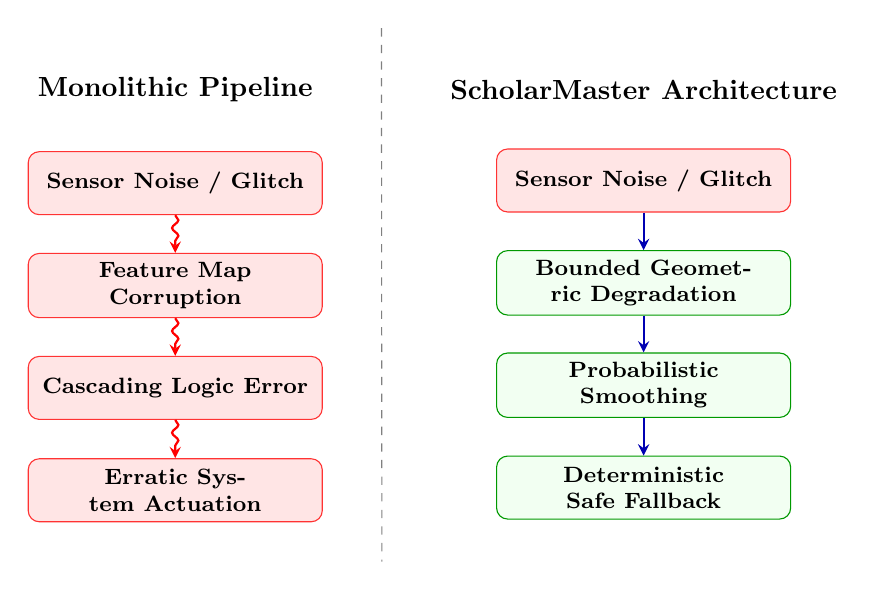
\begin{tikzpicture}[node distance=1.3cm]
  
  % --- LEFT SIDE: MONOLITHIC ---
  \node (M_title) [font=\bfseries] {Monolithic Pipeline};
  \node (M1) [failnode, below=0.5cm of M_title] {Sensor Noise / Glitch};
  \node (M2) [failnode, below of=M1] {Feature Map Corruption};
  \node (M3) [failnode, below of=M2] {Cascading Logic Error};
  \node (M4) [failnode, below of=M3] {Erratic System Actuation};
  
  \draw[failarrow] (M1) -- (M2);
  \draw[failarrow] (M2) -- (M3);
  \draw[failarrow] (M3) -- (M4);

  % --- RIGHT SIDE: SCHOLARMASTER ---
  \node (S_title) [font=\bfseries, right=1.5cm of M_title] {ScholarMaster Architecture};
  \node (S1) [failnode, below=0.5cm of S_title] {Sensor Noise / Glitch};
  \node (S2) [safenode, below of=S1] {Bounded Geometric Degradation};
  \node (S3) [safenode, below of=S2] {Probabilistic Smoothing};
  \node (S4) [safenode, below of=S3] {Deterministic Safe Fallback};
  
  \draw[safearrow] (S1) -- (S2);
  \draw[safearrow] (S2) -- (S3);
  \draw[safearrow] (S3) -- (S4);

  % Divider
  \draw[dashed, gray] ($(M_title.north east) + (0.75cm, 0.5cm)$) -- ($(M4.south east) + (0.75cm, -0.5cm)$);

\end{tikzpicture}
}
\caption{Failure Propagation Comparison. While monolithic systems allow sensor glitches to corrupt global logic, ScholarMaster's boundary invariants force failures to undergo structural containment and safe probabilistic degradation.}
\label{fig:propagation}
\end{figure}

\subsection{Operational Auditability}
Auditability within ScholarMaster emerges structurally from deterministic composition rather than from retrospective logging mechanisms applied after pipeline construction. Because each layer consumes and emits strictly bounded abstractions, a system decision can be reconstructed chronologically without requiring access to raw sensor streams or opaque internal memory states. An auditor can trace the exact geometric abstraction that triggered a specific probability, and the exact probability that satisfied a specific logic predicate.

Table \ref{tab:comparison} summarizes how these emergent properties compare against traditional monolithic designs across key operational dimensions.

\begin{table}[htbp]
\caption{System Property Comparison}
\label{tab:comparison}
\centering
\begin{tabular}{@{}lll@{}}
\toprule
\textbf{Property} & \textbf{Monolith} & \textbf{ScholarMaster} \\
\midrule
Hidden coupling & High & Low \\
Upgrade fragility & High & Low \\
Audit reconstruction & Weak & Strong \\
Failure isolation & Weak & Strong \\
State ownership clarity & Ambiguous & Explicit \\
\bottomrule
\end{tabular}
\end{table}

% ==========================================
% VIII. LIFECYCLE AND DEPLOYMENT REALITIES
% ==========================================
\section{Lifecycle Stability and Upgrade Semantics}
A persistent operational problem observed during longitudinal subsystem development is upgrade fragility. In tightly coupled architectures, updating a perception model frequently invalidates downstream logic assumptions, forcing expensive end-to-end revalidation. Hardware ages, models decay, and systems without isolation eventually become entangled with their oldest component.

ScholarMaster addresses this through admissible-state contracts, an approach that crystallized through iterative subsystem evolution. Internal implementation changes are permitted provided that exported abstraction boundaries remain contract-compliant. This allows individual layers to evolve independently without destabilizing the global system.

For example, during the research program, the geometric sensing subsystem transitioned from a CNN-based detector to a transformer-based representation model without requiring modifications to probabilistic interpretation or logical evaluation layers. As long as the exported geometric abstraction remained compliant with the interface contract, the higher-level reasoning modules were operationally unaware of the implementation shift. This architectural isolation substantially reduces long-term maintenance complexity and helps prevent silent behavioral drift during incremental upgrades.

\section{Institutional Deployment and Multi-Tenant Realities}
Institutional intelligent systems rarely operate in isolation. Universities, hospitals, and industrial facilities frequently require multiple independent operational policies to coexist on shared hardware infrastructure. Experience from deployment-oriented subsystem studies confirmed that functional ownership boundaries are essential for managing this complexity. 

Because operational logic remains isolated from sensing infrastructure, institutions may independently update policy layers without requiring recertification of lower-level perception modules. This separation is especially valuable in regulated environments where governance logic evolves more rapidly than physical sensing hardware. Furthermore, multi-tenant operation becomes feasible because logical evaluation remains isolated from sensing and runtime execution, allowing independent policy domains to operate concurrently without exposing raw sensor streams across organizational boundaries.

This decomposition also permits selective recertification. A modification to institutional logic (e.g., changing attendance compliance rules) does not require re-validation of sensing hardware or probabilistic interpretation models. This substantially reduces operational governance complexity, allowing business logic to iterate faster than physical hardware.

% ==========================================
% IX. CERTIFICATION AND ARCHITECTURAL ECONOMICS
% ==========================================
\section{Certification and Regulatory Implications}
Edge-intelligent deployments increasingly operate under regulatory constraints requiring explainability, auditability, and bounded operational behavior. Certification becomes structurally difficult when perception weights directly influence business logic through entangled intermediate representations---a condition common in monolithic deep-learning systems where functional responsibility cannot be attributed to individual components.

ScholarMaster addresses this by decomposing operational responsibility into independently auditable layers, enabling partial certification of logical or control behavior without requiring full introspection into lower-level sensing internals. The architecture aligns with institutional governance frameworks such as GDPR \cite{b11}, where data minimization and deterministic operational reconstruction are structural requirements rather than optional compliance features.

\section{Architectural Scope, Tradeoffs, and Operational Economics}

ScholarMaster does not attempt to maximize benchmark-specific accuracy metrics or replace tightly coupled inference systems in all deployment contexts. The framework targets environments where auditability, lifecycle maintainability, deterministic composition, and bounded operational behavior take precedence over unconstrained throughput optimization. This scope distinction matters: the architecture intentionally accepts a higher latency floor than fused pipelines in exchange for operational transparency and independent verifiability.

A practical intelligent system is rarely static over its operational lifespan. Heterogeneous hardware drift, version skew between subsystem generations, runtime degradation under aging hardware, serialization overhead accumulation, and institutional deployment heterogeneity present real operational challenges. Cameras fail, microphones degrade, institutional policies evolve, and hardware procurement cycles produce heterogeneous deployments spanning multiple device generations. This reality became increasingly apparent as successive subsystem studies encountered hardware diversity in practice. The architecture is therefore designed under the assumption that evolution is inevitable, prioritizing subsystem survivability under incremental replacement rather than requiring synchronized full-stack upgrades.

Every abstraction boundary in ScholarMaster imposes cost: serialization overhead, interface validation, and stricter ownership constraints. The architecture treats this friction as a stabilizing mechanism---making components harder to connect arbitrarily reduces the surface area for unpredictable coupling failures. Tightly coupled systems frequently appear cheaper during early development because direct memory access minimizes immediate engineering overhead \cite{b17}. However, these short-term economies create maintenance liabilities that compound as the system ages. ScholarMaster externalizes this complexity through explicit interfaces, accepting higher initial discipline requirements in exchange for substantially lower long-term operational cost across upgrades, debugging, auditing, and subsystem replacement within the evaluated architectural constraints.

\subsection{Failed Design Alternatives}
Early architectural prototypes explored shared-memory fusion between the sensing and logic layers, on the premise that raw memory pointers would eliminate serialization copy overhead. The approach reduced end-to-end latency by several milliseconds, but produced hidden coupling: the logic layer became implicitly dependent on the memory layout of the vision pipeline. When the vision model was quantized for deployment, downstream logic failed without any interface contract violation being reported. This experience---among several similar integration episodes---led the architecture to reject shared-memory fusion, accepting serialization overhead as the structural cost of independent verifiability.

\subsection{Hard Architectural Limitations}
This framework is not a universal solution. The architecture intentionally prioritizes modularity and auditability over peak throughput optimization. We explicitly acknowledge the architectural tradeoff: the framework accepts higher latency floors relative to fused pipelines, significant interface-maintenance overhead, increased engineering discipline requirements, and deployment complexity in ultra-low-latency domains. In environments where ultra-low latency dominates all other constraints---such as high-frequency automated trading or low-level drone motor stabilization---tightly coupled, fused pipelines will achieve lower latency bounds. ScholarMaster is explicitly scoped to edge-native domains where interpretability, deterministic containment, and lifecycle maintainability are operationally more valuable than marginal throughput gains.

% ==========================================
% X. CONCLUSION
% ==========================================
\section{Conclusion}
This layered edge-native architecture study demonstrates that scaling intelligent systems at the edge benefits from sustained architectural discipline alongside algorithmic optimization. Formalizing boundary invariants and enforcing abstraction admissibility across the processing pipeline substantially reduces the brittleness that accumulates in monolithic designs over operational lifetimes.

This comes at a cost. Constraining perception, interpretation, logic, and control to interact exclusively through narrow, typed interfaces introduces serialization overhead and engineering friction that fused pipelines avoid. Across the independently validated subsystem studies comprising this research program, however, that friction consistently contributed to failure containment, audit reconstructibility, and independent subsystem evolution---properties that proved more operationally valuable than the marginal latency savings of tighter coupling.

This paper consolidates the systems-engineering understanding that emerged from a multi-paper research trajectory. The resulting framework does not claim universality; it is scoped to edge-native institutional environments where interpretability, deterministic composition, abstraction admissibility, and subsystem survivability under evolution are primary operational requirements. Within that scope, the evidence from independent subsystem validation supports treating enforceable decomposition as a verifiable systems property---one whose enforcement costs are outweighed by the operational transparency and structural resilience it provides.

% ==========================================
% REFERENCES
% ==========================================
\begin{thebibliography}{00}

\bibitem{b1} Z. Zhou, X. Chen, E. Li, L. Zeng, K. Luo, and J. Zhang, "Edge Intelligence: Paving the Last Mile of Artificial Intelligence With Edge Computing," \textit{Proceedings of the IEEE}, vol. 107, no. 8, pp. 1738-1762, 2019.
\bibitem{b2} X. Wang et al., "Convergence of Edge Computing and Deep Learning: A Comprehensive Survey," \textit{IEEE Communications Surveys \& Tutorials}, vol. 22, no. 2, pp. 869-904, 2020.
\bibitem{b3} W. Shi, J. Cao, Q. Zhang, Y. Li, and L. Xu, "Edge Computing: Vision and Challenges," \textit{IEEE Internet of Things Journal}, vol. 3, no. 5, pp. 637-646, 2016.
\bibitem{b4} P. Jamshidi et al., "Microservices: The Journey So Far and Challenges Ahead," \textit{IEEE Software}, vol. 35, no. 3, pp. 24-35, 2018.
\bibitem{b5} E. A. Lee, "The Past, Present and Future of Cyber-Physical Systems: A Focus on Models," \textit{Sensors}, vol. 15, no. 3, pp. 4837-4869, 2015.
\bibitem{b6} H. Kopetz, \textit{Real-Time Systems: Design Principles for Distributed Embedded Applications}. Springer Science \& Business Media, 2011.
\bibitem{b7} M. Bojarski et al., "End to end learning for self-driving cars," \textit{arXiv preprint arXiv:1604.07316}, 2016.
\bibitem{b9} M. Quigley et al., "ROS: an open-source Robot Operating System," in \textit{ICRA workshop on open source software}, 2009.
\bibitem{b10} A. Avizienis, J. Laprie, B. Randell, and C. Landwehr, "Basic concepts and taxonomy of dependable and secure computing," \textit{IEEE Transactions on Dependable and Secure Computing}, vol. 1, no. 1, pp. 11-33, 2004.
\bibitem{b11} P. Voigt and A. von dem Bussche, \textit{The EU General Data Protection Regulation (GDPR): A Practical Guide}. Springer International Publishing, 2017.
\bibitem{b12} D. L. Parnas, "On the criteria to be used in decomposing systems into modules," \textit{Communications of the ACM}, vol. 15, no. 12, pp. 1053-1058, 1972.
\bibitem{b13} M. Satyanarayanan, "The Emergence of Edge Computing," \textit{Computer}, vol. 50, no. 1, pp. 30-39, 2017.
\bibitem{b14} S. Newman, \textit{Building Microservices: Designing Fine-Grained Systems}. O'Reilly Media, Inc., 2015.
\bibitem{b15} J. A. Stankovic, "Research directions for the internet of things," \textit{IEEE Internet of Things Journal}, vol. 1, no. 1, pp. 3-9, 2014.
\bibitem{b16} F. Bonomi, R. Milito, J. Zhu, and S. Addepalli, "Fog computing and its role in the internet of things," in \textit{Proceedings of the first edition of the MCC workshop on Mobile cloud computing}, 2012, pp. 13-16.
\bibitem{b17} D. Sculley et al., "Hidden technical debt in machine learning systems," in \textit{Advances in neural information processing systems}, vol. 28, 2015.
\bibitem{b18} R. Roman, J. Lopez, and M. Mambo, "Mobile edge computing, fog et al.: A survey and analysis of security threats and challenges," \textit{Future Generation Computer Systems}, vol. 78, pp. 680-698, 2018.
\bibitem{b19} Y. Gan et al., "An open-source benchmark suite for microservices and their hardware-software implications for cloud \& edge systems," in \textit{Proceedings of the 24th International Conference on Architectural Support for Programming Languages and Operating Systems (ASPLOS)}, 2019, pp. 3-18.
\bibitem{b20} L. Bass, P. Clements, and R. Kazman, \textit{Software Architecture in Practice}, 3rd ed. Addison-Wesley Professional, 2012.
\bibitem{b21} N. G. Leveson, \textit{Engineering a Safer World: Systems Thinking Applied to Safety}. MIT Press, 2011.

\end{thebibliography}

\end{document}
